\documentclass[professionalfonts]{beamer}
\usepackage[familydefault,light]{Chivo} 
\usepackage[T1]{fontenc}
\usenavigationsymbolstemplate{}
\usepackage[]{hyperref}
\usepackage{tikz,pgf,pgfarrows,pgfnodes,pgfbaseimage}
\graphicspath{{./Pics/}}
\usetikzlibrary{shapes}
\usepackage{setspace}
\newcommand{\evi}[1]{{\colorbox{yellow!50}{{#1}}}}
\newcommand{\exe}[1]{{\color{black!50}{{#1}}}}
\newcommand{\kw}[1]{{\colorbox{black!30}{\color{white}{#1}}}}
\tikzstyle{nd}=[circle,draw=black,thick,minimum size=.8cm,inner sep=1pt]
\setbeamercovered{transparent}
\usetheme{Singapore}
\tikzstyle{nodo}=[ellipse,draw=black!60,fill=black!10,line width=.7pt,minimum width=.7cm,minimum height=.4cm]
\usecolortheme[named=gray]{structure}
\setbeamercolor{block title}{bg=black!20,fg=black}
\setbeamercolor{block body}{bg=black!10,fg=black}

\newif\ifanswers
\answerstrue % comment out to hide answers
%\answersfalse
\ifanswers
\title{Algoritmi Numerici}
\subtitle{Introduzione ed Informazioni Generali}
\else
\title{Numerical Analysis and Optimization}
\subtitle{Introduction and General Information}
\fi
\date{}
\author{Alessandro Antonucci\\{\tt alessandro.antonucci@supsi.ch}}
\begin{document}
\maketitle
\frame{\frametitle{\ifanswers Il corso \else Class \fi}
\setstretch{1.4}
\begin{itemize}
\item 6 ECTS
\item \ifanswers Ore settimanali: 2 (teoria) + 2 (esercitazioni)\\entrambi i semestri \else Hours per week: 2 (theory) + 2 (exercise)\\both semesters \fi
\item \ifanswers Docente: \else Instructor: \fi Alessandro Antonucci (theory)\\
{\tt email/teams: alessandro.antonucci@supsi.ch} 
\item \ifanswers Esercitazioni: \else Esercises: \fi 
\end{itemize}
\begin{center}
\ifanswers
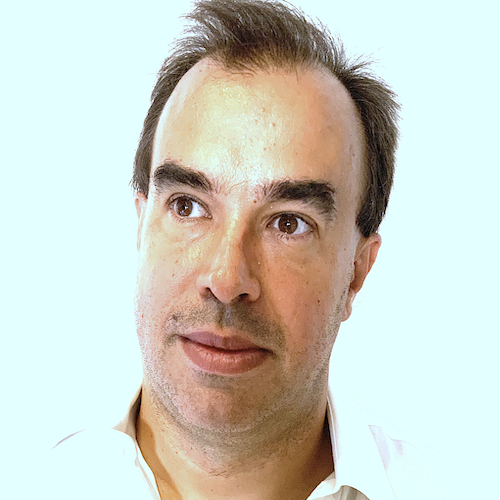
\includegraphics[width=2cm]{alessandro}
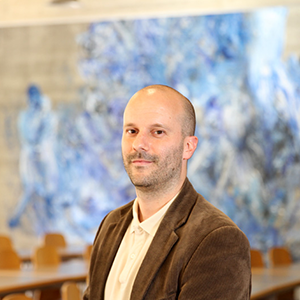
\includegraphics[width=2cm]{lorenzo}
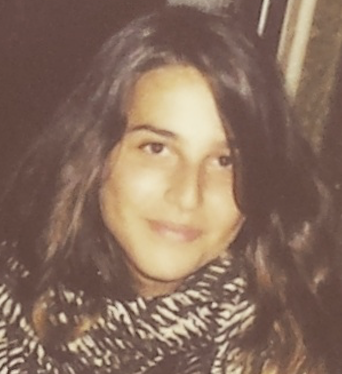
\includegraphics[width=2cm]{lilith}
\\
Antonucci \quad Camponovo \quad Mattei\\
Alessandro \quad Lorenzo \quad Lilith
\else
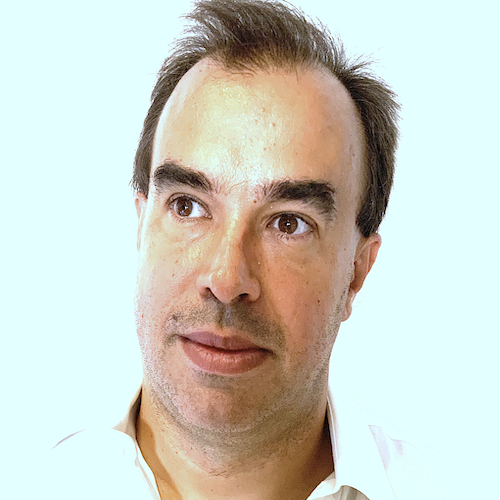
\includegraphics[width=2cm]{alessandro}
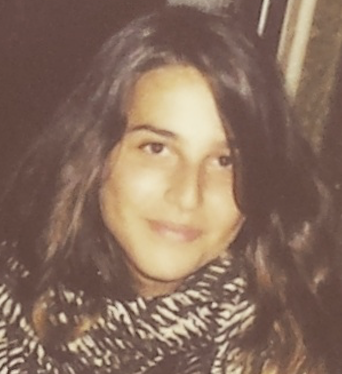
\includegraphics[width=1.8cm]{lilith}
\\ \small
Antonucci \quad Mattei\\
Alessandro \quad Lilith
\fi
\end{center}}

\frame{\frametitle{\ifanswers Orario \else Schedule\fi}
\begin{center}
\ifanswers 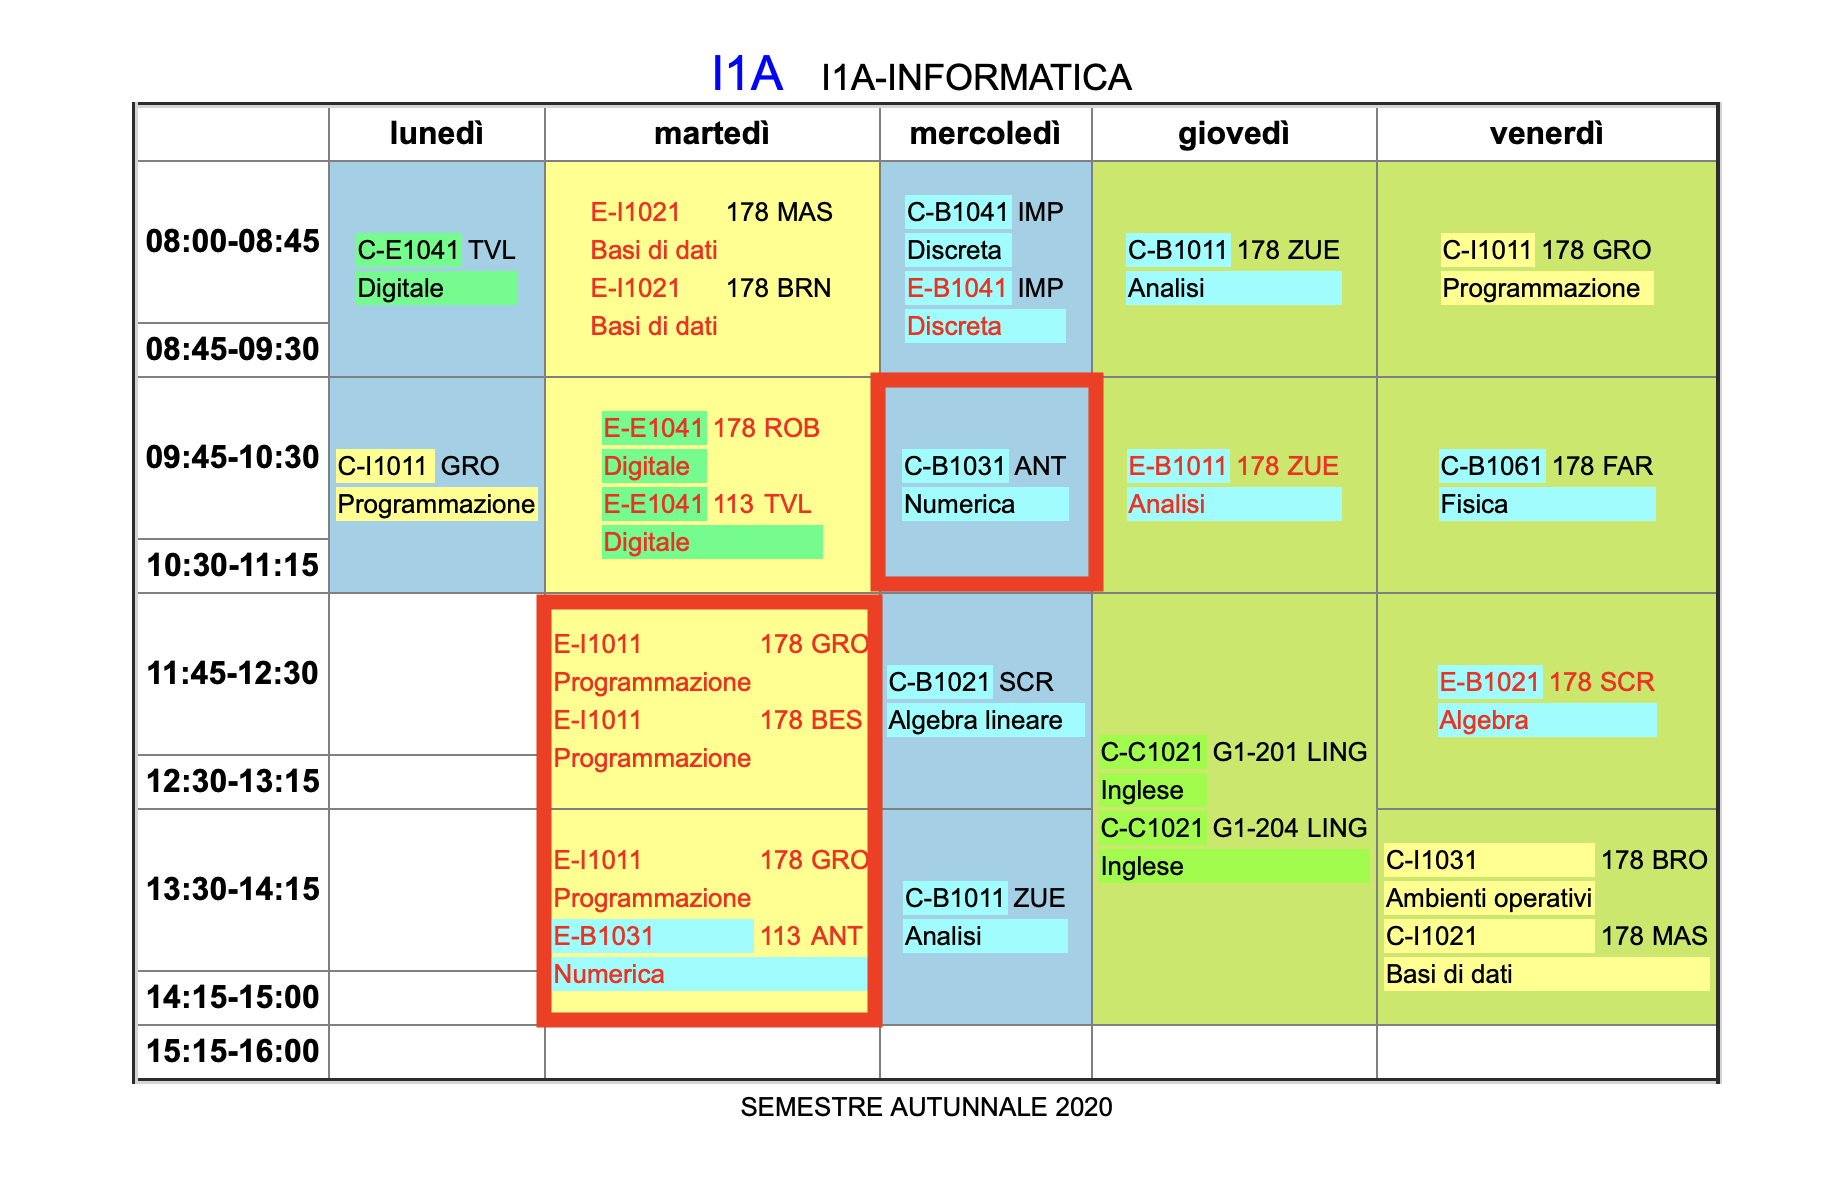
\includegraphics[width=5.2cm,height=5cm]{i1a}
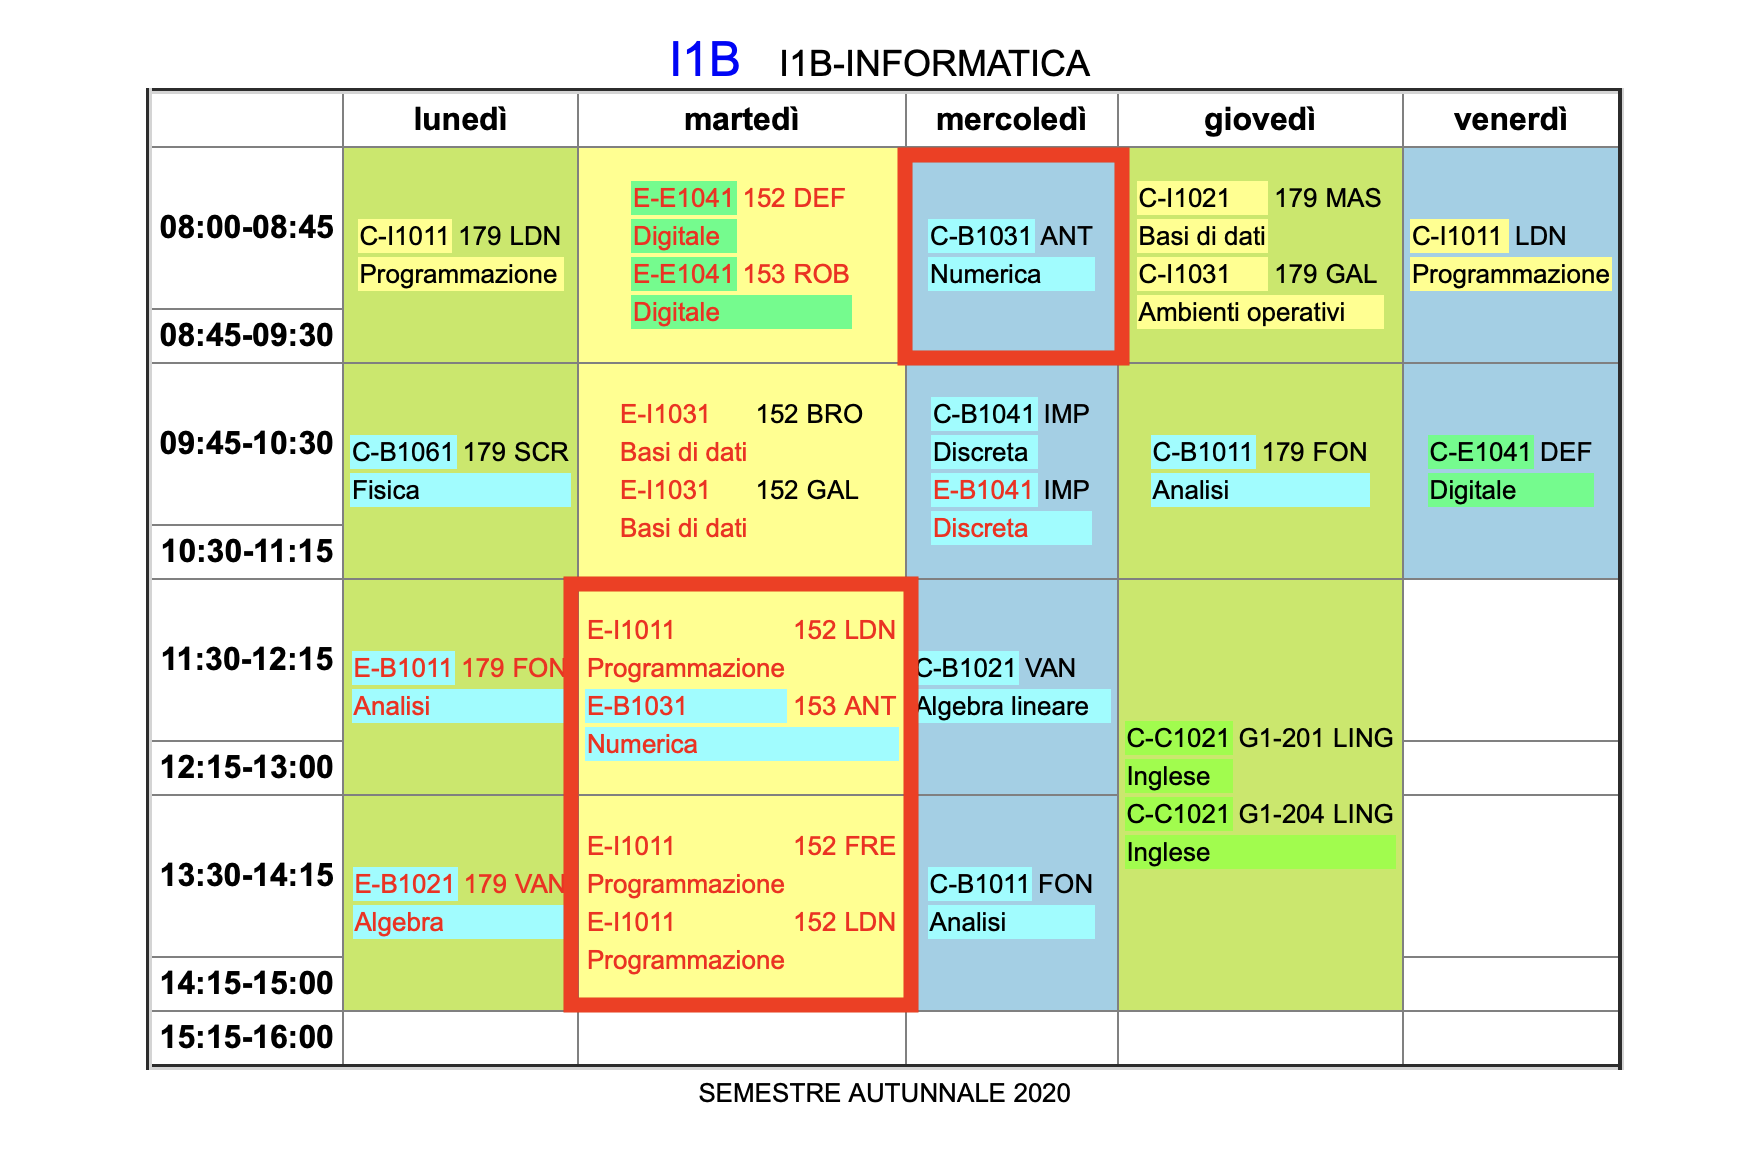
\includegraphics[width=5.2cm,height=5cm]{i1b}
\else 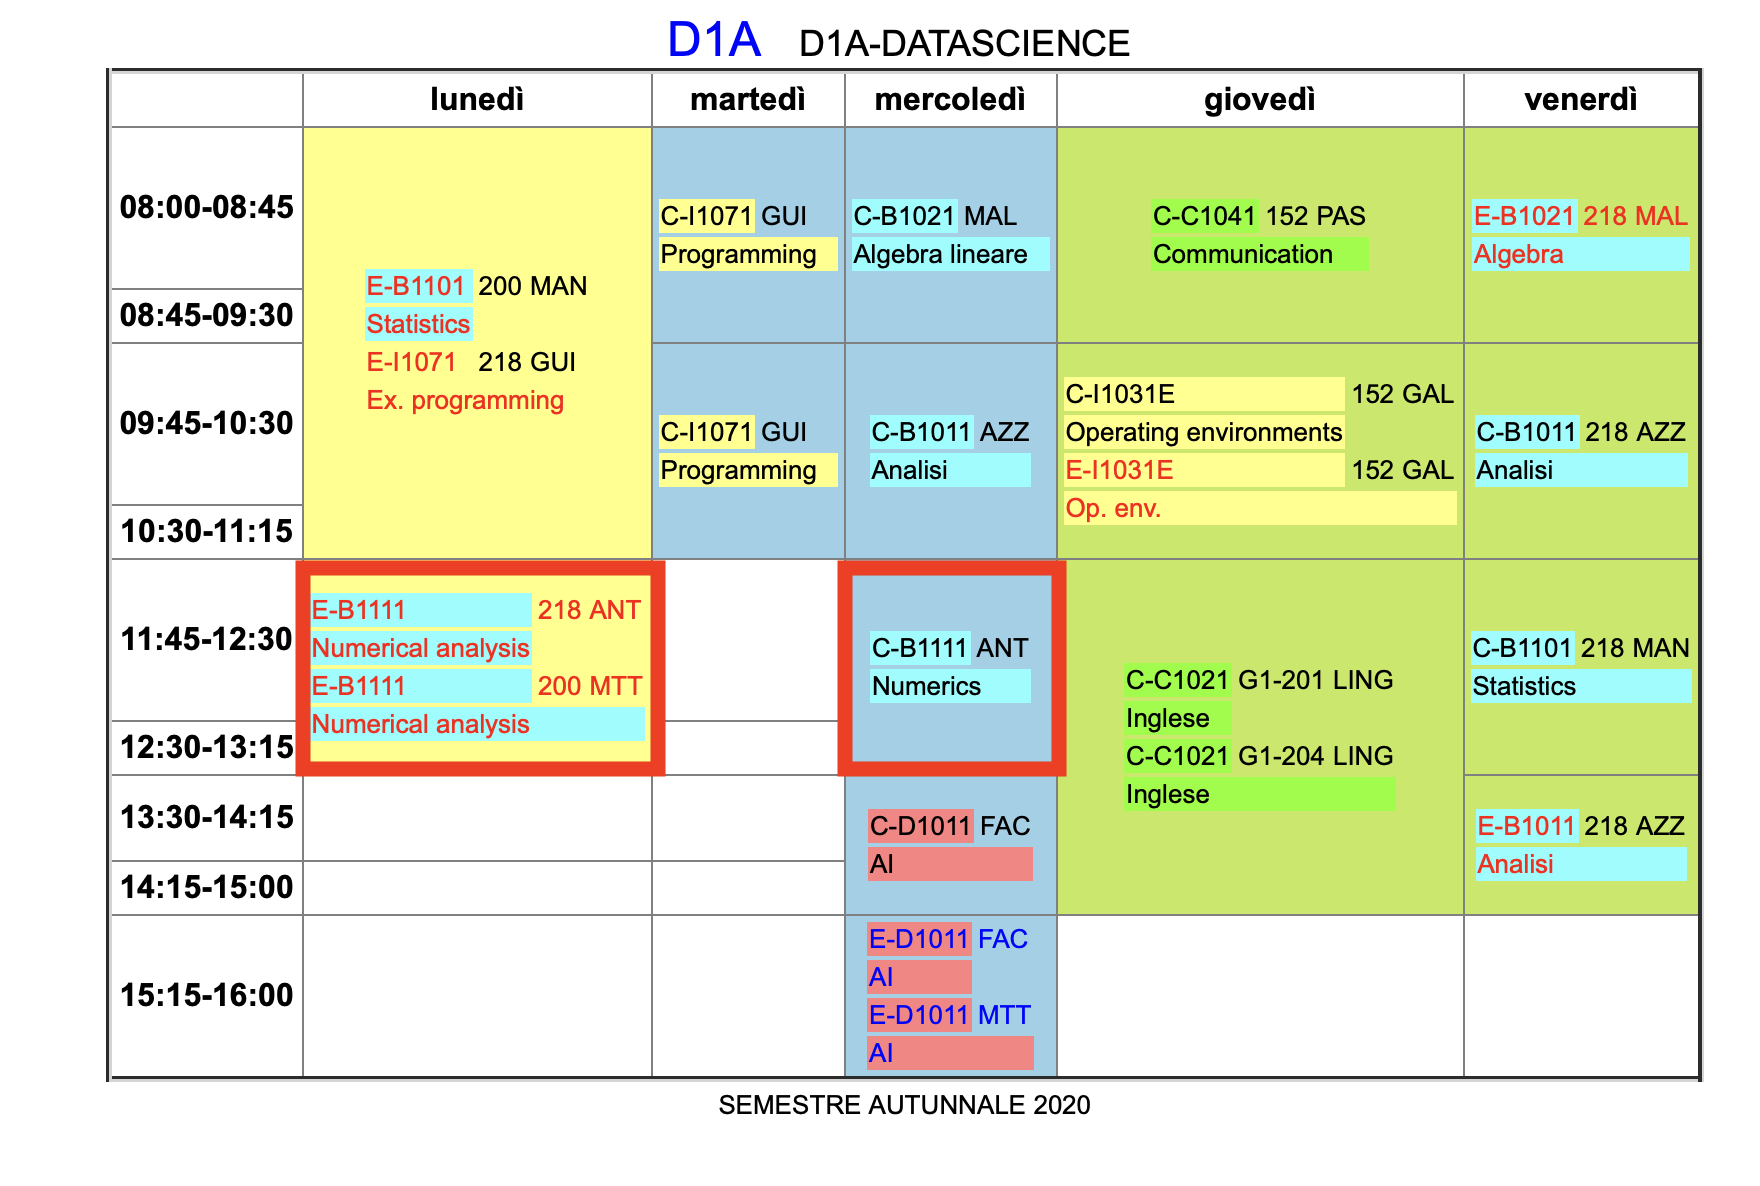
\includegraphics[width=10cm,height=7cm]{ds}
\fi
\end{center}}


\frame{\frametitle{\ifanswers Contenuti e Prove Scritte \else Topics and Tests \fi}
\begin{tabular}{ll}
\ifanswers
{\small Sett-Nov}&Rappresentazioni del numero\\
{\small Nov-Gen}& Risoluzione equazioni non-lineari\\
&\\
&{\small Gen 13, 2021 :: TEST \# 1}\\
&\\
{\small Feb-Apr}& Risoluzione di sistemi di equazioni lineari\\
{\small Apr-Giu}& Interpolazione ed integrazione numerica\\
&\\
&{\small Giu (seconda settimana), 2021 :: TEST \# 2}\\
\else
{\small :: Sept-Nov ::}&Representing Numbers with Computers\\
{\small :: Nov-Jan ::}& Solving Non-Linear Equations\\
&\\
&{\small Jan 13, 2021 :: TEST \# 1}\\
&\\
{\small :: Feb-Apr ::}& Solving Linear Systems\\
{\small :: Apr-Jun :: }& Interpolation and Optimization\\
&\\
&{\small Jun (1st or 2nd week), 2021 :: TEST \# 2}\\
\fi
\end{tabular}}


\frame{\frametitle{\ifanswers Valutazioni \else Grades \fi}

\begin{itemize}
\item $(n_1,n_2)$ := \ifanswers note test (\#1 e \#2)\else grades of tests (\#1 and \#2) \fi
\item $\min_{i=1,2} n_i \geq 6$ (\ifanswers ambizioso\else ambitious\fi)
\item $(n_1\geq 4) \wedge (n_2\geq 4) $ (\ifanswers dignitoso\else fair\fi)
\item $\sum_{i=1}^2 n_i \geq 8$ (\ifanswers minimale\else minimal\fi)
\end{itemize} 
\vskip 5mm
\begin{center}
\ifanswers
Test Open-book\\ {\small riassunto su due fogli A4 (4 facciate)}
\else
Open-book Tests\\ {\small(you can bring a summary made of\\two A4 sheets corresponding to 4 pages)}
\fi
\end{center}
}

\frame{\frametitle{\ifanswers Scopo del Corso \else Course Goal \fi}
\begin{columns}
\begin{column}[T]{0.5\textwidth}
\ifanswers
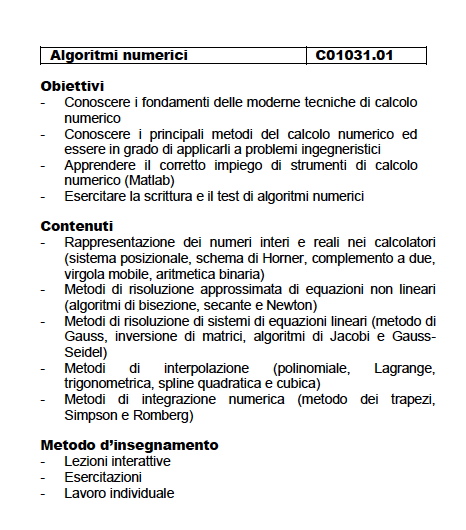
\includegraphics[width=6cm]{Piano}
\else
\includegraphics[width=6cm]{Goals}
\fi
\end{column}
\begin{column}[T]{0.5\textwidth}
\vskip 5mm
\ifanswers 
Come da piano di studio
\else
See study plan
\fi
\vskip 5mm
\ifanswers Ma anche:
\begin{itemize}
\item Formalizzare problemi in maniera algoritmica
\item Gestire complessit\`a tecnica nei calcoli
\item ``Svelare'' questioni legate alla rappresentazione dei numeri ed alla risoluzione di problemi mediante calcolatore
\end{itemize}
\else
But also:
\begin{itemize}
    \item Algorithmic Thinking
    \item Complexity Control
    \item ``Reveal'' what computers can do (numbers representations/solvers)
\end{itemize}
\fi
\end{column}
\end{columns}}



\frame{\frametitle{\ifanswers Presenze \else Attendance \fi}
\setstretch{1.3}
\begin{itemize}
\item \ifanswers Modulo iCorsi per presenze \else Instructor records attendances in iCorsi\fi
\item \ifanswers In caso di assenza mandare una mail/teams al docente\\(se possibile prima della lezione) \else If unable to join the class, send an email/teams to alessandro.antonucci@supsi.ch (before or after)\fi
\item \ifanswers 
E-mail e Teams accounts {\tt @student.supsi.ch} = strumento di comunicazione col docente
\else
E-mail and Teams account {\tt @student.supsi.ch} are important communication tools \\(be able to check them frequently)
\fi
\item 
\ifanswers
Inizio lezione puntuale, no ritardi se non giustificati
\else
Classes will start on time, timeliness is important!
\fi
\end{itemize}}


\frame{\frametitle{Tools}
\setstretch{1.3}
\begin{itemize}
\item iCorsi
\item Teams
\item Forum (@ iCorsi)
\item Python (Colab), Excel, Geogebra, Kahoot, $\ldots$ 
\end{itemize}}
\end{document}



